\documentclass[11pt]{article}
\usepackage[margin=0.75in]{geometry}
\usepackage{amsmath,amsthm,amssymb}
\usepackage{graphicx}
\usepackage{enumitem}
\usepackage{listings}
\usepackage{mathptmx}
\usepackage{comment}
\usepackage{multirow}
\usepackage{gensymb}
\usepackage{wrapfig}
\lstset{
  basicstyle=\ttfamily,
  mathescape
}



\begin{document}

\title{CS 301 Lab Report 1}
\author{Sebastien James, Michael Hernandez-Thomas}
\date{\today}
\maketitle

\section*{ABSTRACT}
This lab report covers the second lab of CS 301. Now that we are acquainted with the workings of the platform used in class, we design two forms of control: reactive control and feedback control. To this end, two new behaviors are needed: a reactive behavior to perform different actions based on a number of hand waves, and a looping feedback behavior to maintain the robot at a set distance from the wall. 

\begin{comment}

Summarize the report. A good rule of thumb: 1-2 sentences on each of Sections I-IV. (Emphasis on Sections I and II.)
\end{comment}

\section*{I. INTRODUCTION}

In this lab, we explore the challenges and uses of different controls. Now that we know how to move the robot, we need a means to control those actuators to accomplish tasks. These tasks involve moving the robot in a precise and calculated manner to achieve a desired state. This state can either be an achievement goal, like turning to a fixed direction, or a maintenance goal, like keeping a certain distance from the wall while walking. Both types of goals are needed to design a functional robot. However, there are cases where the robot needs to quickly and efficiently react to its environment. In this case, we would have a reactive system, where the robot makes changes quickly without modeling its environment.

To this end, we make two behaviors, one reactive control and one feedback closed-loop control. 
Initially, the reactive control was supposed to be in response to the robot encountering obstacles while walking, but because of technical problems with having multiple sonars, the behavior was instead changed to turning based on the number of waves in front of its sonar. (less reactive, wait). 
The second behavior is having the robot follow a wall while maintaining a certain distance from it. This behavior is closed-loop, as we constantly are measuring the distance from the wall and trying to maintain that distance goal.

\begin{comment}
Introduce the topic of the lab assignment. Use terminology from the readings. Explain:
Why it is important?
What about it is challenging?
Do not yet talk about your specific approach, nor any experimental results.
Cite the readings (and any other books/papers/sites) as appropriate.
Examples of going above and beyond: Consulting references outside of the course material. Demonstrating a
particularly deep understanding or synthesis of information.
Suggested length: 1 page.

Discuss what role does control play on a robot, and why is it important; what is open/closed loop control; what is reactive control; and all at a level of detail where specific controllers and how do they operate are discussed.
\end{comment}

\section*{II. METHODS}

The lab can be divided in two major parts: a first where we are tasked with developing a walking a turning gait to be used in the more complex behaviors of the second part.

Our first task was to create a forward walking gait. We started from the one we developed in the previous lab assignment. The legs are divided into two groups to keep three feet on the ground at all times. However, while the gait was fast, it did not walk straight. We found that the robot tended to rotate to the right after a few steps because of the left front foot sliding when planted while the right foot stayed in place when planted. To counter this drift, we pulled the front left ankle joint inwards to create for friction. We also found that the more inward it points, the more the robot turns to the left.

Next, we needed a turning gait. Our turning gait from the first lab was almost an exact 90 degree turn, so we spent a little time tweaking the amount it turns by to get as close as possible to a 90 degree turn. Otherwise the gait was the same: set the robot down, rotate the legs, and push back up.

For the reactive control, we were tasked with making a behavior that reacts to the amount of hand waves. We started by making a hand-detection method: the robot first waits for the distance its sonar measures to be less than 10 cm. Then it waits for the distance to be above 50 cm, since the hand wave goes past the sensor. It then waits for up to 4 seconds for more hand waves. Each wave adds one to a counter, which determines what the robot should do: 1 wave makes the robot turn right, 2 waves is turn left, and 3 is turn around. 



Finally, our feedback closed-loop control behavior is wall following. We first mounted a new sonar on the right side of the robot to have it facing the wall while the robot walks forward. The robot then starts its feedback loop. At every step, it measures the distance between it and the wall. To counteract the noise the sensor gives, we take 10 measurements over the course of 0.1 seconds, then take the median value. We then compare that value to the distance measured at the start. The robot then used proportional control to steer itself: the larger the difference, the more it bends the front right and middle right ankles. This equates to more or less of a turn to the left, away from the wall. 

\begin{wrapfigure}{r}{0.35\textwidth}
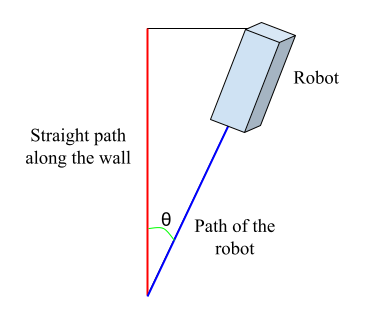
\includegraphics[width=0.35\textwidth]{trig.png}
\centering
\end{wrapfigure}

If the amount the robot needs to turn by is more than just adjusting the limb positions can correct for, the robot then calculates how much it needs to turn by calculating the angle between its path and the path perpendicular to the wall. To calculate $\theta$, we keep track of how far the robot has walked (blue line), and we calculate the black line as follows: 

\[ |distance_{target} - distance_{measured} |\] 

\[\theta = \text{arcsin}(\frac{distance}{path})\]

The loop then repeats. \\



To assess the accuracy of these behaviors, we also need to set up measurement tests. 

For the standard walking gait, we measured the final distance traveled and the offset from the center line. Learning from last lab, we marked where the legs should be at the start, so the robot shouldn't have any large deviations due to us mispositioning the robot at the start. We performed five trials of 5, 10, and 15 seconds each, measuring with a meter stick.

For the turning gait, we measured the heading offset and time of execution over five trials of turning left, right, and around. For the time we just used a phone timer, and for the angle we used two crossing meter sticks and a protractor to measure the angle offset.

Similarly to the walking test, we performed five trials of 5, 10, and 15 seconds each for the wall following behavior. We measured the distance travelled and the distance to the wall, again with a meter stick.




\begin{comment}

Describe in detail your approach to solving the lab's challenge. Include a thorough description of any developed processing/algorithms, that covers:
The sensor input, and sensor processing.
The algorithm reasoning.
The actuation output.
(This description should be at a conceptual level, and should not describe the low-level details of your code.)
Provide a clear and convincing motivation for your approach.
Cite the readings (and any other books/papers/sites) as appropriate.
Clearly describe the experimental tests you will run to empirically validate your approach.
Explain why these tests were chosen. (What will the tests show?)
Examples of going above and beyond: An algorithm or hardware design that is particularly clever, or more complex to implement.
Suggested length: 1-2 pages.

Make sure to provide a thorough description of your implementation of each of Steps 1, 2, 5, and 7.
Make sure also to clearly present, and motivate, the measures that will be collected in Steps 3 and 8.

\end{comment}

\section*{III. RESULTS}

\subsection*{Forward walking gait}

The robot was places on the same tape markers on the floor each time, ensuring no error was introduced by misplacing it. The robot was then run, and the distances were measured using meter sticks.

\begin{figure}[h!]
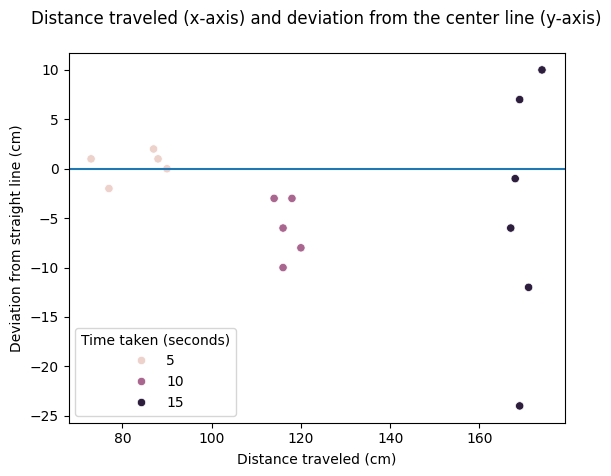
\includegraphics[width=140mm]{walk.png}
\centering
\end{figure}

\subsection*{Turning gait}

For measuring the turning error, we set the robot on marks on the ground to consistently place it in the same spot. After running the program for turning, we used two crossed meter sticks to get the angle measured. 

For the time of execution, we always measured 7 seconds for both the left and right turn, and 14 seconds for turning around.

\begin{figure}[h!]
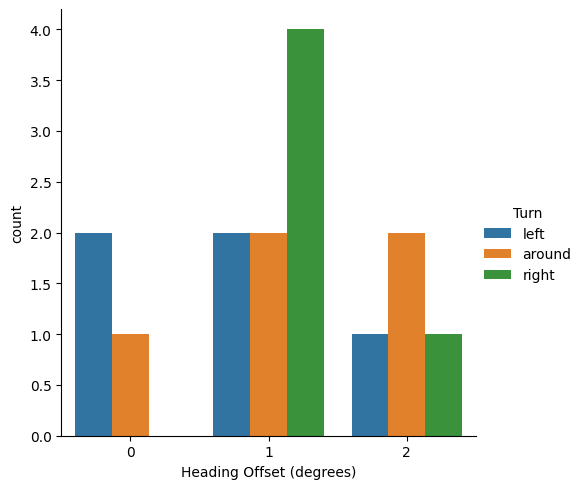
\includegraphics[width=140mm]{offset.png}
\centering
\end{figure}

\subsection*{Wall following}

Finally, for the wall following, we placed the robot at 35cm from the wall, measured from the edge of the chassis. The program was then run, automatically stopping after the required time. We then used meter sticks to measure the distance travelled perpendicular to the wall as well as the final distance from the wall.

\begin{figure}[h!]
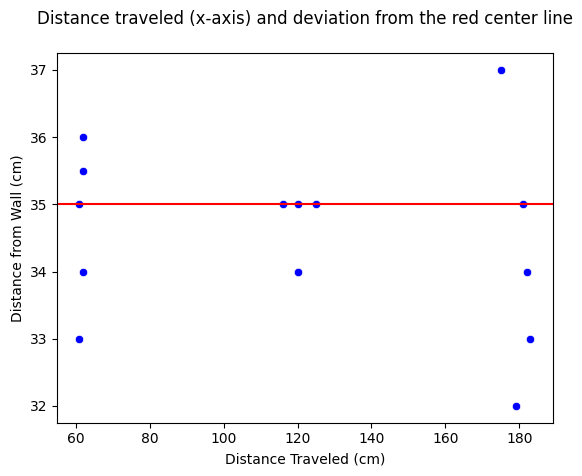
\includegraphics[width=120mm]{wall.png}
\centering
\end{figure}

\begin{comment}

Report the data collected and analyzed from your experimental testing.
Make sure to label all axes, define variables/parameters, give units for all variables, title plots.
Clearly describe the details of your experimental conditions and data collection techniques.
(Under what conditions was a measurement performed, and using what measurement tool?)
Include statistics, figures and tables, as appropriate.
The presentation of your data should be concise and thorough. For example, displaying multiple experimental conditions on the same plot is often easier for the reader to digest, and as a bonus also takes up less space.
Examples of going above and beyond: Gathering an extra type of experimental data.
Suggested length: 1-2 pages.

Be sure to describe any relevant initial conditions, measurement mechanisms, etc. (How was distance measured?
Angles? What was the testing environment?)

\end{comment}

\section*{IV. DISCUSSION}

Walking was definitely the most challenging of the lab. Our current walk gait has a problem with sliding. Since the front and back hip motors are angled offset from the chassis, the feet are set down and dragged on the floor in a circular arc, causing them to slide somewhat unpredictably. This can explain why the 5 and 10 second measurements are about the same distance off the center line, but over the course of 15 seconds the robot accumulates error and ends up on both sides of the center line. 

However, the error is small enough that having a feedback loop to correct it leads to a relatively stable forward walking gait. Following the wall keeps the robot within $\pm$ 3cm instead of deviating 20 cm off.

The hand-waving turning behavior isn't completely reactive, since it needs to wait for more input before executing the behavior. It also does build somewhat of a model of a hand wave, contrasting the definition in the book of a reactive behavior.

I would like to improve the walking gait, specifically to have the robot not need to have external references to know where it is. Ideally, the robot would be able to set down its foot in a location, and keep it there while swinging its body over the foot like a living creature would.

One other aspect to improve would be to change our turning gait to not have to go all the way down, turn, and come back up, as it is time consuming. As it is now, any small adjustment up to 45 degrees to the left or right will take 7 seconds, even if the turn is only 10 degrees. This would probably mean switching to a similar pattern as the walking gait, with 3 legs on the floor while moving the other 3.

\begin{comment}
Provide a discussion of your observed results, and any insights you have gained about the lab topic.
Don't just repeat the data reported in the RESULTS section, but rather provide a higher-level analysis of your observed results.
What were the positive results?
Are there any key aspects of your approach that accounted for them?
Where is there room for improvement: with respect to the empirical results, data collection, algorithm, etc?
How do your results change/support the way you look at the lab topic (with respect to its perceived challenges,
importance within the field, etc.)?
Examples of going above and beyond: Demonstrating particularly deep insight or observations.
Suggested length: 1-2 pages

Discuss the performance of each of your developed behaviors.
How accurate do you expect each of your measurements are, and why?
What are some potential sources of noise and/or uncertainty?

Identify any reasons for poor performance, sources of uncertainty, areas for improvement; in any of Steps 1-8.

\end{comment}
\section*{V. CONCULSION}
The behaviors developed explore different used of control. Reactive control is used to determine what action to take in the hand-waving behavior. Feedback control is used for the wall following behavior. Additional work can be done on the standard walking gait to ensure it keeps straight.




\begin{comment}
Recap the report. A good rule of thumb: 1-3 sentences to each of Sections II-IV. (Emphasis on Sections III and IV.
\end{comment}

\section*{REFERENCES}

Matarić, M. J. (2008). The Robotics Primer. The MIT Press. 

\end{document}